% This is "aamas2016_sample.tex", a revised version of aamas2015_sample.tex
% This file should be compiled with "aamas2016.cls"
% This example file demonstrates the use of the 'aamas2015.cls'
% LaTeX2e document class file. It is intended for those submitting
% articles to the AAMAS-2016 conference. This file is based on
% the sig-alternate.tex example file.
% The 'sig-alternate.cls' file of ACM will produce a similar-looking,
% albeit, 'tighter' paper resulting in, invariably, fewer pages
% than the original ACM style.
%
% ----------------------------------------------------------------------------------------------------------------
% This .tex file (and associated .cls ) produces:
%       1) The Permission Statement
%       2) The Conference (location) Info information
%       3) The Copyright Line with AAMAS data
%       4) NO page numbers
%
% as against the acm_proc_article-sp.cls file which
% DOES NOT produce 1) through 3) above.
%
% Using 'aamas2015.cls' you don't have control
% from within the source .tex file, over both the CopyrightYear
% (defaulted to 20XX) and the IFAAMAS Copyright Data
% (defaulted to X-XXXXX-XX-X/XX/XX).
% These information will be overwritten by fixed AAMAS 2015  information
% in the style files - it is NOT as you are used to with ACM style files.
%
% ---------------------------------------------------------------------------------------------------------------
% This .tex source is an example which *does* use
% the .bib file (from which the .bbl file is produced).
% REMEMBER HOWEVER: After having produced the .bbl file,
% and prior to final submission, you *NEED* to 'insert'
% your .bbl file into your source .tex file so as to provide
% ONE 'self-contained' source file.
%


\documentclass{aamas2016}
\usepackage{graphics} % for pdf, bitmapped graphics files
\usepackage{comment}
\usepackage{amsmath,amssymb,amsxtra,amsfonts}%,comment}
% The following packages can be found on http:\\www.ctan.org
\usepackage{graphics} % for pdf, bitmapped graphics files
\usepackage{epsfig} % for postscript graphics files
\usepackage{amsfonts}
\usepackage{url}
\usepackage{comment}
\usepackage{color}
\usepackage{threeparttable}
%\usepackage{algorithmic}
\usepackage{algorithmicx}
\usepackage{algpseudocode}
\usepackage{algorithm}
% Mathematics
\newcommand{\iforget}{\displaystyle}
\newcommand\Nat{\mathbb{N}}
\renewcommand\natural{\mathbb{N}}
\newcommand\rot{\mathbb{S}}
%% Math defs
% The set of reals, integers, etc.
\renewcommand{\Re}{\mathbb{R}}
\newcommand{\Ze}{\mathbb {Z}}
\newcommand{\Pe}{\mathbb {P}}
\newcommand{\I}{\mathcal{I}}                                                          

% \newcommand{\qed}{\hfill \ensuremath{\Box}}
\newcommand{\blambda}{\boldsymbol\lambda}
\newcommand{\bLambda}{\boldsymbol\Lambda}
\newcommand{\bpsi}{\boldsymbol\psi}
\newcommand{\bPsi}{\boldsymbol\Psi}
\newcommand{\hatE}{\hat{\mathbb{E}}_{N}}

\newtheorem{proposition}{Proposition}
% \newenvironment{proof}[1][Proof]{\begin{trivlist}
% \item[\hskip \labelsep {\bfseries #1}]}{\end{trivlist}}
\newtheorem{assumption}{Assumption}
\newtheorem{corollary}{Corollary}
\newtheorem{remark}{Remark}
\newtheorem{lemma}{Lemma}

\DeclareMathOperator*{\argmin}{argmin}

% if you are using PDF LaTeX and you cannot find a way for producing
% letter, the following explicit settings may help

\usepackage{bm}
%\usepackage{mathrsfs}

\usepackage{xspace}
\newcommand{\etal}{et~al.\xspace} 

\pdfpagewidth=8.5truein
\pdfpageheight=11truein

\begin{document}

% In the original styles from ACM, you would have needed to
% add meta-info here. This is not necessary for AAMAS 2015  as
% the complete copyright information is generated by the cls-files.


\title{{\color{red} Lifelong Learning Applications in Mobile Robotics} }

% AUTHORS


% For initial submission, do not give author names, but the
% tracking number, instead, as the review process is blind.

% You need the command \numberofauthors to handle the 'placement
% and alignment' of the authors beneath the title.
%
% For aesthetic reasons, we recommend 'three authors at a time'
% i.e. three 'name/affiliation blocks' be placed beneath the title.
%
% NOTE: You are NOT restricted in how many 'rows' of
% "name/affiliations" may appear. We just ask that you restrict
% the number of 'columns' to three.
%
% Because of the available 'opening page real-estate'
% we ask you to refrain from putting more than six authors
% (two rows with three columns) beneath the article title.
% More than six makes the first-page appear very cluttered indeed.
%
% Use the \alignauthor commands to handle the names
% and affiliations for an 'aesthetic maximum' of six authors.
% Add names, affiliations, addresses for
% the seventh etc. author(s) as the argument for the
% \additionalauthors command.
% These 'additional authors' will be output/set for you
% without further effort on your part as the last section in
% the body of your article BEFORE References or any Appendices.

%\numberofauthors{8} %  in this sample file, there are a *total*
% of EIGHT authors. SIX appear on the 'first-page' (for formatting
% reasons) and the remaining two appear in the \additionalauthors section.
%

\numberofauthors{7}

% \author{
% % You can go ahead and credit any number of authors here,
% % e.g. one 'row of three' or two rows (consisting of one row of three
% % and a second row of one, two or three).
% %
% % The command \alignauthor (no curly braces needed) should
% % precede each author name, affiliation/snail-mail address and
% % e-mail address. Additionally, tag each line of
% % affiliation/address with \affaddr, and tag the
% % e-mail address with \email.
% % 1st. author
% David Isele\\
% % 2nd. author
% \alignauthor
% Jos\'e Marcio Luna\\
% % 3rd. author
% \alignauthor Eric Eaton
% \and  % use '\and' if you need 'another row' of author names
% \alignauthor
% \affaddr{University of Pennsylvania}\\
%       \affaddr{3330 Walnut St}\\
%       \affaddr{Philadelphia, PA 19104}\\
%       \email{\{isele,joseluna,eeaton\}@seas.upenn.edu}
% \and
% \alignauthor Gabriel de la Cruz\\
% % 5th. author
% \alignauthor James Irwin\\
% % 6th. author
% \alignauthor Brandon Kallaher\\
% % 7th. author
% \alignauthor Matthew Taylor\\
% \and
% \alignauthor
%       \affaddr{Washington State University}\\
%       \affaddr{P.O. Box 642752}\\
%       \affaddr{Pullman, WA 99164}\\
%       \email{\{gabriel.delacruz,james.irwin,brandon.kallaher.taylor\}@wsu.edu}
% }


\author{
% You can go ahead and credit any number of authors here,
% e.g. one 'row of three' or two rows (consisting of one row of three
% and a second row of one, two or three).
%
% The command \alignauthor (no curly braces needed) should
% precede each author name, affiliation/snail-mail address and
% e-mail address. Additionally, tag each line of
% affiliation/address with \affaddr, and tag the
% e-mail address with \email.
% 1st. author
David Isele\\
\affaddr{University of Pennsylvania}\\
      \affaddr{3330 Walnut St}\\
      \affaddr{Philadelphia, PA 19104}\\
      \email{isele@seas.upenn.edu}
% 2nd. author
\alignauthor
Jos\'e Marcio Luna\\
\affaddr{University of Pennsylvania}\\
      \affaddr{3330 Walnut St}\\
      \affaddr{Philadelphia, PA 19104}\\
      \email{joseluna@seas.upenn.edu}
% 3rd. author
\alignauthor Eric Eaton\\
\affaddr{University of Pennsylvania}\\
      \affaddr{3330 Walnut St}\\
      \affaddr{Philadelphia, PA 19104}\\
      \email{eeaton@seas.upenn.edu}
\and  % use '\and' if you need 'another row' of author names
% 4th. author
\alignauthor Gabriel de la Cruz\\
      \affaddr{Washington State University}\\
      \affaddr{P.O. Box 642752}\\
      \affaddr{Pullman, WA 99164}\\
      \email{gabriel.delacruz@wsu.edu}
% 5th. author
\alignauthor James Irwin\\
      \affaddr{Washington State University}\\
      \affaddr{P.O. Box 642752}\\
      \affaddr{Pullman, WA 99164}\\
      \email{james.irwin@wsu.edu}
% 6th. author
\alignauthor Brandon Kallaher\\
      \affaddr{Washington State University}\\
      \affaddr{P.O. Box 642752}\\
      \affaddr{Pullman, WA 99164}\\
      \email{brandon.kallaher@wsu.edu}
\and
% 7th. author
\alignauthor Matthew Taylor\\
      \affaddr{Washington State University}\\
      \affaddr{P.O. Box 642752}\\
      \affaddr{Pullman, WA 99164}\\
      \email{taylor@eecs.wsu.edu}
}

%\and
%% 7th. author
%\alignauthor Lawrence P. Leipuner\\
%       \affaddr{Brookhaven Laboratories}\\
%       \affaddr{Brookhaven National Lab}\\
%       \affaddr{P.O. Box 5000}\\
%       \email{lleipuner@researchlabs.org}

%% 8th. author
%\alignauthor Sean Fogarty\\
%       \affaddr{NASA Ames Research Center}\\
%       \affaddr{Moffett Field}\\
%       \affaddr{California 94035}\\
%       \email{fogartys@amesres.org}

%% 9th. author
%\alignauthor Charles Palmer\\
%       \affaddr{Palmer Research Laboratories}\\
%       \affaddr{8600 Datapoint Drive}\\
%       \affaddr{San Antonio, Texas 78229}\\
%       \email{cpalmer@prl.com}

%}


% \alignauthor
% Paper XXX
%Ben Trovato\titlenote{Dr.~Trovato insisted his name be first.}\\
%       \affaddr{Institute for Clarity in Documentation}\\
%       \affaddr{1932 Wallamaloo Lane}\\
%       \affaddr{Wallamaloo, New Zealand}\\
%       \email{trovato@corporation.com}
% 2nd. author
%\alignauthor
%G.K.M. Tobin\titlenote{The secretary disavows any knowledge of this author's actions.}\\
%       \affaddr{Institute for Clarity in Documentation}\\
%       \affaddr{P.O. Box 1212}\\
%       \affaddr{Dublin, Ohio 43017-6221}\\
%       \email{webmaster@marysville-ohio.com}
% 3rd. author
%\alignauthor Lars Th{\o}rv{\"a}ld\titlenote{This author is the one who did all the really hard work.}\\
%       \affaddr{The Th{\o}rv{\"a}ld Group}\\
%       \affaddr{1 Th{\o}rv{\"a}ld Circle}\\
%       \affaddr{Hekla, Iceland}\\
%       \email{larst@affiliation.org}
% }

%\and  % use '\and' if you need 'another row' of author names

% 4th. author
%\alignauthor Lawrence P. Leipuner\\
%       \affaddr{Brookhaven Laboratories}\\
%       \affaddr{Brookhaven National Lab}\\
%       \affaddr{P.O. Box 5000}\\
%       \email{lleipuner@researchlabs.org}

% 5th. author
%\alignauthor Sean Fogarty\\
%       \affaddr{NASA Ames Research Center}\\
%       \affaddr{Moffett Field}\\
%       \affaddr{California 94035}\\
%       \email{fogartys@amesres.org}

% 6th. author
%\alignauthor Charles Palmer\\
%       \affaddr{Palmer Research Laboratories}\\
%      \affaddr{8600 Datapoint Drive}\\
%       \affaddr{San Antonio, Texas 78229}\\
%       \email{cpalmer@prl.com}

%\and

%% 7th. author
%\alignauthor Lawrence P. Leipuner\\
%       \affaddr{Brookhaven Laboratories}\\
%       \affaddr{Brookhaven National Lab}\\
%       \affaddr{P.O. Box 5000}\\
%       \email{lleipuner@researchlabs.org}

%% 8th. author
%\alignauthor Sean Fogarty\\
%       \affaddr{NASA Ames Research Center}\\
%       \affaddr{Moffett Field}\\
%       \affaddr{California 94035}\\
%       \email{fogartys@amesres.org}

%% 9th. author
%\alignauthor Charles Palmer\\
%       \affaddr{Palmer Research Laboratories}\\
%       \affaddr{8600 Datapoint Drive}\\
%       \affaddr{San Antonio, Texas 78229}\\
%       \email{cpalmer@prl.com}

%}

%% There's nothing stopping you putting the seventh, eighth, etc.
%% author on the opening page (as the 'third row') but we ask,
%% for aesthetic reasons that you place these 'additional authors'
%% in the \additional authors block, viz.
%\additionalauthors{Additional authors: John Smith (The Th{\o}rv{\"a}ld Group,
%email: {\texttt{jsmith@affiliation.org}}) and Julius P.~Kumquat
%(The Kumquat Consortium, email: {\texttt{jpkumquat@consortium.net}}).}
%\date{30 July 1999}
%% Just remember to make sure that the TOTAL number of authors
%% is the number that will appear on the first page PLUS the
%% number that will appear in the \additionalauthors section.

\maketitle

\begin{abstract}
Learning controllers for heterogeneous multi-agent systems is often an expensive process when controllers for each system are learned individually. Advances in lifelong learning suggest that information between systems can be shared, improving the quality of the controllers that are learned. However these results have been largely theoretical, with applications limited to benchmark problems with known dynamics. We show that these methods can be extended to robotic platforms. Particularly we validate our assumptions for transfer learning between tasks in order to carry out a disurbance rejection problem.

\end{abstract}

% Note that the category section should be completed after reference to the ACM Computing Classification Scheme available at
% http://www.acm.org/about/class/1998/.

\category{{\color{red} H.4}}{{\color{red} Information Systems Applications}}{{\color{red} Miscellaneous}}

%A category including the fourth, optional field follows...
%\category{D.2.8}{Software Engineering}{Metrics}[complexity measures, performance measures]

%General terms should be selected from the following 16 terms: Algorithms, Management, Measurement, Documentation, Performance, Design, Economics, Reliability, Experimentation, Security, Human Factors, Standardization, Languages, Theory, Legal Aspects, Verification.

\terms{{\color{red} Delphi theory}}

%Keywords are your own choice of terms you would like the paper to be indexed by.

\keywords{{\color{red} AAMAS proceedings, \LaTeX, text tagging}}

\section{Introduction}

%Motivation
Given differences in manufacturing and wear, even identically designed robots may require very different control policies. Learning a unique control policy for each robot in the system can be very costly. One approach to reduce the amount of learning is to share information between robots. Lifelong learning \cite{Ruvolo2013} is a promising approach for accomplishing transfer because it allows the different systems to be encountered consecutively rather than requiring all the systems and models be available prior to training. Also it preserves and possibly improves the models encountered early on, as opposed to transfer methods which only optimize for the new system.
% Learning on robotic systems is a very costly process. The time needed to run learning algorithms often prohibits running the large number of trials needed to learn a robust model. %, and physical systems wear down from repeated trials often changing the system over time. This problem is greatly exacerbated in multirobot systems which can contain many possibly different systems, each of  which may have a different objective, and therefore may require learning a unique controller for each agent in the system.


% State of the Art
Most work in lifelong learning has focused largely on theory, using benchmark simulations to demonstrate their results \cite{Ruvolo2013,BouAmmar2014a,bouAmmar2015unsupervised}. The few examples of lifelong learning on robots focus in skill refinement on a single robot \cite{thrun1995lifelong} \cite{kleiner2002towards} rather than sharing information across multiple robots. 
%Work in multitask learning has shown that performance can be improved by sharing data between tasks. Recent advances in lifelong learning show that knowledge sharing can be handled efficiently in an online manner, re\cite{Ruvolo2013}moving the restriction that data be collected for all tasks before optimization can take place. However these methods are often demonstrated on simulated systems with known dynamics and parameterizations. 

%transfer citations \cite{barrett2010transfer} \cite{chalup2007machine}

% Disturbance Rejection
The contribution of this work is to present the first results of lifelong learning a on real robots.
{\color{red} We apply the PG-ELLA framework \cite{BouAmmar2014a} to the problem of disturbance rejection as a step towards solving fault tolerant control problems.}

% We propose a lifelong learning method that can learn controllers in the presence of unknown disturbances that differ from task to task. Unlike most previous work in lifelong learning, we demonstrate this method on Turtlebots, an affordable robotics platform.  

\section{Background} \label{background}
As mentioned before, the current work focuses on learning transfer for reinforcement learning tasks. However, it can be easily extended
to th esupervised learing case, \emph{e.g.,} regression and classification problems. In this section we cover the mathematical framework that
supports our experiments on lifelong learning.

\subsection{Reinforcement Learning}

In reinforcement Learning (RL) and agent must select sequential actions to maximize its expected return. RL approaches do not 
require previous knowledge of the system dynamics, instead, the control policies are learned through the interactions with the system.
RL problems are typically formalized as Markov Decision Processes (MDPs) with the form $\langle \mathcal{X}, \mathcal{A}, P, R, \gamma \rangle$ where
$\mathcal{X}\subset\Re^{d_{x}}$ is the set of states, $\mathcal{A}$ is the set of actions, 
$P:\mathcal{X}\times \mathcal{A}\times \mathcal{X}\rightarrow [0,1]$ is the state transition probability describing the systems dynamics.
$R:\mathcal{X}\times \mathcal{A} \rightarrow \Re$ is the reward function and $\gamma \in [0,1)$ is the reward discount factor. At each time 
step $h$, the agent is in the state $\mathbf{x}_{h} \in \mathcal{X}$ and must choose an action $\mathbf{a}_{h} \in \mathcal{A}$ so that
it transitions to a new state $\mathbf{x}_{h+1}$ with state transition probability 
$P(\mathbf{x}_{h+1}|\mathbf{x}_{h},\mathbf{a}_{h})$, thus yielding 
a reward $r_{h}$ according to $R$. The action is selected according to a policy $\pi:\mathcal{X}\times \mathcal{A} \rightarrow [0,1]$ which
specifies a probability distribution over actions given the current state. The goal of RL is to find the optimal policy $\pi^{*}$ 
that maximizes the expectation of the per-step reward.

In Policy Gradient (PG) methods [], the policy is represented as a function defined over a parameter vector 
$\boldsymbol{\theta} \in \Re^{d_{\theta}}$ that provides the gains of the control inputs of the system. The goal of PG is to optimize
the expected average return,
\begin{equation}
 \mathcal{J}(\boldsymbol{\theta})=\int_{\mathbb{T}}p_{\boldsymbol{\theta}}(\tau)\mathcal{R}(\tau)\mbox{d}\tau,
 \label{retPG}
\end{equation}
where $\mathbb{T}$ is the set of all trajectories and $\mathcal{R}(\tau)$ is the average per-step reward, specifically,
\begin{eqnarray}
 p_{\boldsymbol{\theta}} & = & \prod_{h=0}^{H}p(\mathbf{x}_{h+1}|\mathbf{x}_{h},\mathbf{a}_{h})\pi(\mathbf{a}_{h},\mathbf{x}_{h}) \nonumber \\
 \mathcal{R}(\tau) & = & \frac{1}{H}\sum_{h=0}^{H} r(\mathbf{s}_{h},\mathbf{a}_{h},\mathbf{s}_{h+1}) \nonumber
\end{eqnarray}

The optimization of the policy is carried out by comparing trajectories generated by a policy $\pi_{\boldsymbol{\theta}}$ with those
generated by a new policy $\pi_{\boldsymbol{\tilde{\theta}}}$. For more details see [].

\subsection{Finite Differences and Policy Search}
The local optimization around existing policies $\pi$ parameterized by a parameter vector $\boldsymbol{\theta}$ 
is carried out by computing changes in the policy parameters $\boldsymbol{\Delta \theta}$ that will increase the expected reward, thus
producing the iterative update,
\begin{displaymath}
 \boldsymbol{\theta}_{m+1} = \boldsymbol{\theta}_{m}+\boldsymbol{\Delta \theta}_{m}.
\end{displaymath}

{\color{red}More methods to be added here taken from the survey paper.}

Gradient-based methods for policy updates follow the gradient of the expected return $\mathcal{J}$ {\color{red}check the notation for the return
and the difference between return and reward} given a step-size $\alpha$ {\color{red} in case we talk about the minimizer of the KL
divergence which is alpha as well},
\begin{displaymath}
 \boldsymbol{\theta}_{m+1} = \boldsymbol{\theta}_{m}+\alpha\nabla_{\boldsymbol{\theta}}\mathcal{J}.
\end{displaymath}

In finite difference gradients, we have a set of $k$ {\color{red} are we using k for anything else?} perturbed policy parameters are
assessed to estimate the gradient as follows,
\begin{displaymath}
 \Delta\hat{\mathcal{J}}_{\mathbf{p}} \approx \mathcal{J}(\boldsymbol{\theta}_{m}+\boldsymbol{\Delta\theta_{p}}) - \mathcal{J}_{ref},
\end{displaymath}
where $\mathbf{p}=[1,\ldots,k]$ are the individual perturbations, $\Delta\hat{\mathcal{J}}_{\mathbf{p}}$ is the estimate of their 
effect on the return, and the $\mathcal{J}_{ref}$ is a reference return which is usually taken as the return of the unperturbed
parameters. By using linear regression we get an approximation of the gradient,
\begin{displaymath}
 \nabla_{\boldsymbol{\theta}}\mathcal{J} \approx \left(\boldsymbol{\Delta\Theta^{T}\Delta\Theta}\right)^{-1}\boldsymbol{\Delta\Theta}^{T}\Delta\boldsymbol{\hat{J}_{p}}.
\end{displaymath}
where $\Delta\boldsymbol{\hat{J}_{p}}$ contains all the stacked samples of $\Delta\hat{\mathcal{J}}_{\mathbf{p}}$ and  $\boldsymbol{\Delta\Theta}$
contains the ones of $\boldsymbol{\Delta\theta_{p}}$. This approach is sensitive to the type and magnitude of the perturbations, as well as
to the step size $\alpha$. Since the number of perturbations needs to be as large as the number of parameters, this method is
considered to be noisy and inefficient for problems with large sets of parameters.

\subsection{Lifelong Learning}

Lifelong learning focuses on learning a set of tasks consecutively while performing well across all tasks. Given a round 
$t = 1,\dots,t_{\max}$ a task $T^{(t)}$ is observed. This task is defined acccording to the learning problem in place, \emph{e.g.,}
regression and classification. We assume that the model associated to $T^{(t)}$ is parameterized
by a parameter vector $\boldsymbol{\theta}^{(t)} \in \Re^{d_{\theta}}$. The ideal goal is that prior knowledge about tasks 
$T^{(1)},\ldots,T^{(t-1)}$ should provide enough information so that the lifelong learning algorithm performs better and faster on $T^{(t)}$
while being able to scale as the number of tasks increases.

Based on [Kumar,Ruvolo], we assume there is a shared basis $\boldsymbol{L}\in \Re^{d_{x}\times l}$ {\color{red} I changed notation 
for hidden layers} and a sparse weight vector $\boldsymbol{s}^{(t)}\in \Re^{\l}$, so that the parameter $\boldsymbol{\theta}^{(t)}$
is given by,
\begin{displaymath}
 \boldsymbol{\theta}^{(t)}=\boldsymbol{Ls}^{(t)}.
\end{displaymath}

Using the return function for PG in (\ref{retPG}) we propose the following multitask objective function,
\begin{displaymath}
 \argmin_{\boldsymbol{L},\boldsymbol{S}}\frac{1}{|\boldsymbol{T}|}\sum_{t}\left[ -\mathcal{J}(\boldsymbol{\theta}^{(t)}) + \lambda \| \boldsymbol{s}^{(t)} \|_{1} \right] + \mu\|\boldsymbol{L}\|_{F}^{2},
\end{displaymath}
where $\boldsymbol{S}$ is the set of the sparse vectors $\boldsymbol{s}^{(t)}$, the L1 norm of $\| \boldsymbol{s}^{(t)} \|_{1}$ 
provides sparse code for $\boldsymbol{s}^{(t)}$ and the Frobenious norm in $|\boldsymbol{L}\|_{F}^{2}$ provides regularization. The
coefficients $\mu$ and $\lambda \in \Re$ are weights for the regularization and sparsity respectively.

The learning objective function is approximated by a second order Taylor expansion around the single task policy, and the optimization
problem is solved by using the online ELLA algorithm introduced in \cite{Ruvolo2013} and extended for the reinforcement learning setting using Policy
Gradients (PG) in \cite{BouAmmar2014a}. However, PG relies on the indirect maximization of the return function based on the maximization of a lower bound.
Although this bound has reportedly been tight enough to guarantee maximization of the return function, we chose to use finite
differences to search the optimal policy to make sure we maximize the return function directly. {\color{red} We could summarize 
the vectorized update rules of PG-ELLA as in the zero transfer paper.}

\section{Experiments} \label{Experiments}
{\color{red} This definitely needs more work. Some printscreen of gazeo an a picture of the turtlebot would be good. Some technical description
of the robot would complement the ideas here as well.}


\begin{figure}[!htbp]
    \centering
        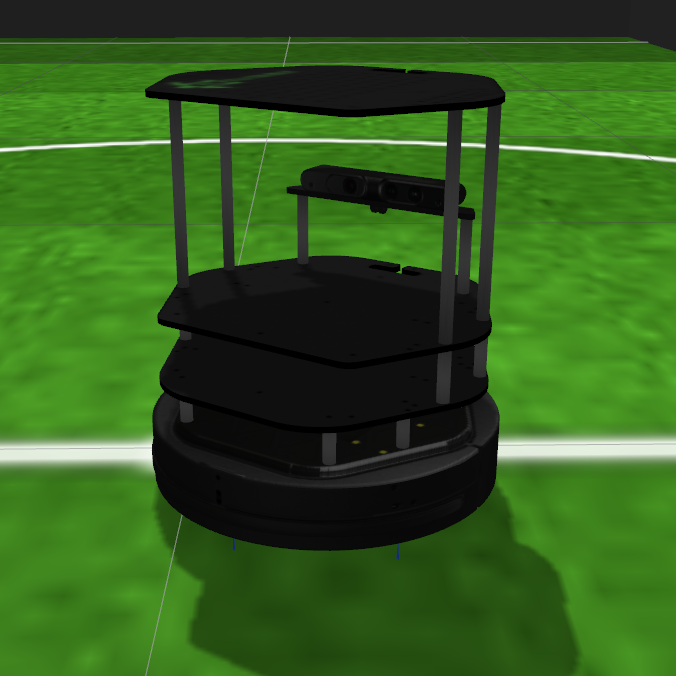
\includegraphics[width=.3\textwidth]{images/turtlebot_crop.png}
        \caption{Turtlebot in Gazebo Simulator. }\label{fig:numfeat}
\end{figure}

We evaluated our approach by modelling the control policies for different turtlebot systems. Turtlebots are an afforable robotics 
platform that uses the robot operating system ROS and includes a simulator in Gazebo. We artifically create a collection of different 
turtlebots by applying a constant disturbance to the control signal. Each turtlebot has a different constant disturbance drawn 
uniformly from $[-.1, .1]$. The turtlebot has a $\mathbb{R}^4$ state and an $\mathbb{R}^2$ action following the model of 
Aicardi \etal \cite{aicardi1994closed} which describes the state as: {\color{red} I can verify this model and possibly try to get a better 
illustrative image.}

\begin{equation} \label{eqn:state}
	%\bm{x}^{(t)} \!=\! \begin{bmatrix} r cos(\alpha) & \alpha & \frac{cos(\alpha)sin(\alpha)}{\alpha}\left(\alpha + \kappa + \phi \right) & 1 \end{bmatrix} \enspace
	\bm{x} \!=\! \begin{bmatrix} r cos(\alpha) \\ \alpha \\ \frac{cos(\alpha)sin(\alpha)}{\alpha}\left(\alpha + \kappa + \phi \right) \\ 1 \end{bmatrix} \enspace
\end{equation}

{\color{red} it's important to make sure that we aren't reusing notation.}
where $r$ is the distance to the goal, $\alpha$ is the difference between heading angle and the robot and the goal, $\psi$ is the angle of the robot with respect to the global coordinate frame and $\kappa$ is the desired angle. 

\begin{figure}[!htbp]
    \centering
        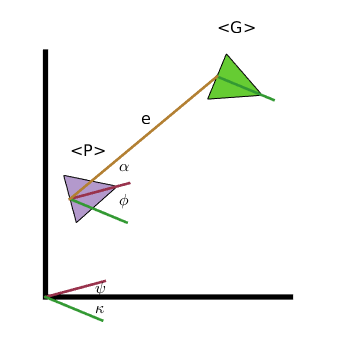
\includegraphics[width=.3\textwidth]{images/model.png}
        \caption{Problem for go to goal task. }\label{fig:numfeat}
\end{figure}

The state is a non-linear transformation of the position and heading angle (?). We were not able to learn a linear policy on this non-linear state transformation using either the natural actor critic \cite{peters2008natural} or episodic REINFORCE \cite{williams1992simple} policy gradient methods.   

\subsection{Methodology} 
We start by generating 20 robots, each with a different constant disturbance and a unique goal, both selected uniformly. The experiments were run for 50 time steps. 15 rollouts were generated for each learning iteration and $\theta^*$ was taken from the single task learner policy after 20 iterations. This is fewer iterations than is required for any system to converge to a good controller. 

We learned a dictionary with $k=8$, and compare the learning time of a single task finite difference policy versus the learning time of a system using ELLA.
% use identity as hessian 


\begin{figure}[!htbp]
    \centering
        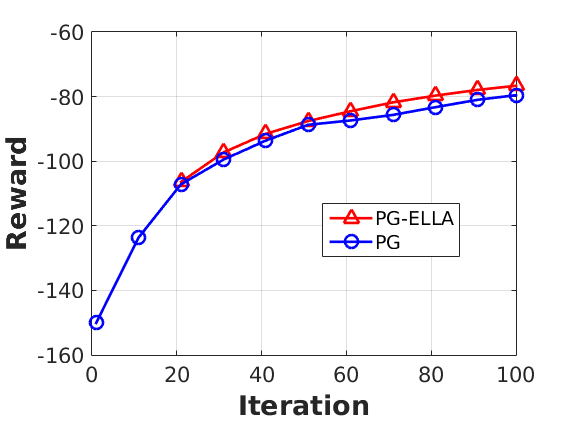
\includegraphics[width=.3\textwidth]{images/2016_2_3_reward.png}
        \caption{Learning curves for finite differences and finite differences using ELLA to transfer information between tasks. }\label{fig:numfeat}
\end{figure}

\begin{figure}[!htbp]
    \centering
        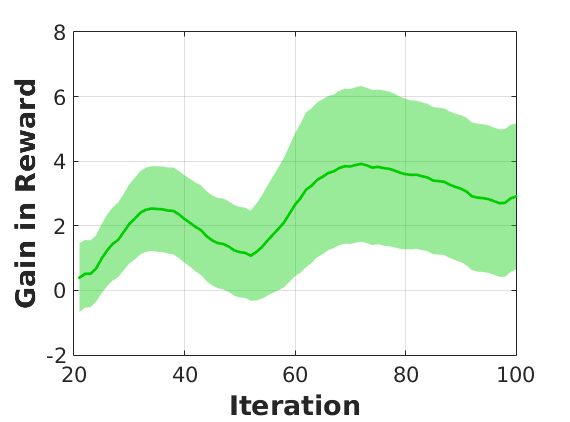
\includegraphics[width=.3\textwidth]{images/2016_2_3_gain.png}
        \caption{The positive transfer achieved by using ELLA. }\label{fig:numfeat}
\end{figure}



\section{Conclusions}
{\color{red} there aren't conclusions yet.}
This paragraph will end the body of this sample document.
Remember that you might still have Acknowledgments or
Appendices; brief samples of these
follow.  There is still the Bibliography to deal with; and
we will make a disclaimer about that here: with the exception
of the reference to the \LaTeX\ book, the citations in
this paper are to articles which have nothing to
do with the present subject and are used as
examples only.
%\end{document}

%Acknowledgements are optional
\section*{Acknowledgments}
{\color{red} 
This section is optional; it is a location for you
to acknowledge grants, funding, editing assistance and
what have you.  In the present case, for example, the
authors would like to thank Gerald Murray of ACM for
his help in codifying this \textit{Author's Guide}
and the \textbf{.cls} and \textbf{.tex} files that it describes.
}
%
%APPENDICES are optional
%\balancecolumns
\appendix
%Appendix A
\section{Headings in Appendices}
{\color{red} 
The rules about hierarchical headings discussed above for
the body of the article are different in the appendices.
In the \textbf{appendix} environment, the command
\textbf{section} is used to
indicate the start of each Appendix, with alphabetic order
designation (i.e. the first is A, the second B, etc.) and
a title (if you include one).  So, if you need
hierarchical structure
\textit{within} an Appendix, start with \textbf{subsection} as the
highest level. Here is an outline of the body of this
document in Appendix-appropriate form:
\subsection{Introduction}
\subsection{The Body of the Paper}
\subsubsection{Type Changes and  Special Characters}
\subsubsection{Math Equations}
\paragraph{Inline (In-text) Equations}
\paragraph{Display Equations}
\subsubsection{Citations}
\subsubsection{Tables}
\subsubsection{Figures}
\subsubsection{Theorem-like Constructs}
\subsubsection*{A Caveat for the \TeX\ Expert}
\subsection{Conclusions}
\subsection{Acknowledgments}
\subsection{Additional Authors}

}

%
% For AAMAS-2016, as references are unlimited but appendices must fit within
% 8 pages, the References section must come after the appendices (if any)
%
% The following two commands are all you need in the
% initial runs of your .tex file to
% produce the bibliography for the citations in your paper.

\bibliographystyle{abbrv}
{\color{red} Reference section requires a lot more work.}
\bibliography{sigproc}  % sigproc.bib is the name of the Bibliography in this case
% You must have a proper ".bib" file
%  and remember to run:
% latex bibtex latex latex
% to resolve all references
%
% ACM needs 'a single self-contained file'!
%\balancecolumns % GM June 2007
% That's all folks!
\end{document}
